\chapter{Integration Notes}

\section{Integration into a Project}
%\ifnum \DocumentGroup=1{
%Please refer to the installation instructions included in the RTA-SUM Getting Started Guide to generate the \LongName directly inside ISOLAR-AB.
%Briefly you can select RTA Code Generator for configuring the SUM Modules that want to be integrated in the project accordigly to its Model Year (MY) version. 
%When the option "Not Configured" is selected, the module will not be integrated.
%}
%\else
%{
There is no need for standard installation procedure for TCS. The folder itself contains all the necessary
artifacts to integrate into a project. Dropping the complete folder structure into a BSW configuration
project will enable the user to configure TCS and generate all the necessary artifacts.
%}
%\fi

\section{Module Dependencies}

\paragraph{NVM - SumTCSInitValue}
In order to fulfill the requirement to store the \code{SumTCSInitValue} in memory, a RAM mirror block is used for storing this data in non-volatile memory.
It is assumed the user will configure the NVM stack to support this required information.
Further, it is expected that during shutdown, the appropriate BSW services will write that specific NVM block to persistent storage if battery voltage is good to perform NVM write operation.

\paragraph{COM - MasterClockSignal}
Assumptions are made about the COM configuration which is used in conjunction with this module.
Specifically, COM must be configured to provide the Master Clock Signal to the defined \LongName interface \code{COM_MasterClockSignal}.

\paragraph{TimeSyncMessage}
The resolution of a \code{TimeSyncMessage} is 100 ms.
This is equal to saying that the timestamp in the \code{TimeSyncMessage} is a counter representing the number of 100 ms increments.
It follows that the 36 bits of the \code{TimeSyncMessage} can represent up to $2^{36} \cdot 100$ ms (approximately 6.872E9 seconds, 79536 days, 217 years).

\paragraph{Exlusive Areas}
 In order to prohibit concurrent data access, RTA-SUM TCS configures each runnable \newline to use the \code{RunsInsideExclusiveArea} protection.
 
\paragraph{TCS\_Init}
 As specified in SDV-8002, the TCS provides an initialization routine \code{TCS_Init} that must be invoked at start-up by the BswM or by runnbale \code{Runnable_TCS_Init}.

\section{Configuring TCS} 
Once the complete package has been added to your project, an additional module \LongName should appear.
From here you can open and start to configure the module.
Specific descriptions of each configurable parameter are available in the “Description” view of
%\ifnum \DocumentGroup=1{
%ISOLAR-B
%}
%\else
%{ 
ISOLAR-A with BCT add-on
%}\fi 
when a parameter is selected and also in the section \nameref{sec:confparams} of this document.

\section{Generating Artifacts}
Generating the C/H/SWCD files from your configuration is similar to other BSW modules delivered from ETAS.
The Code Generation perspective of the 
%\ifnum \DocumentGroup=1{
%ISOLAR-B
%}
%\else
%{ 
ISOLAR-A with BCT add-on
%}\fi
should present the user with a dialog to select specific module within the project to generate.
%\ifnum \DocumentGroup=1{
%%Nothing
%}
%\else
%{ 
Either a Partial Build or Full Build can be used, depending on the needs of the user.
%}\fi
In case of any configuration errors present in RTA-SUM TCS, the console window will output a description of any errors found during generation.
Further, when the user is configuring the module, the Problems Log will show any active errors in the configuration of RTA-SUM TCS.
A third visual aid is the appearance of red X’s in the configuration view over items which are invalid.
Simply hovering over these X’s will provide the user a description of the problem.
These are static validations.

After generating the SUM files, execute the MemMap tool to generate memory mapping file of the module (\file{SUM\_TCS\_MemMap.h}).

\section{Configuring the RTE}
After the user has configured and generated the artifacts for \LongName, the output SWCD file \linebreak(\file{SUM\_TCS\_Cfg\_SWCD.arxml}) can be used for the RTE configuration.
This is a complete SWC description per the AUTOSAR standard of all the users configured ports and interfaces required for the project specific configuration.
This SWCD is a standard ASW component and not a module description.
Therefore, there are no special considerations to be taken into account when configuring the RTE.
It is recommended that if specific changes are required to the SWCD, the user not manually edit this file, rather update and regenerate the configuration with the required changes.

Note: RTE command used for RTE generation

\begin{rtecommandline}
-nts --samples=memmap --os-define-osenv=RTAOS40 --exclusive-area-optimization=disable --os-output-param=all --strict-unconnected-rport-check=off
\end{rtecommandline}


\chapter{Module Configuration}

\section{Configuration Parameters}
\label{sec:confparams}

\subsection{Container - TcsGeneral}
The configuration structure of the \LongName consists of one container named \textbf{TcsGeneral} with few configuration parameters as you can see in the picture below.

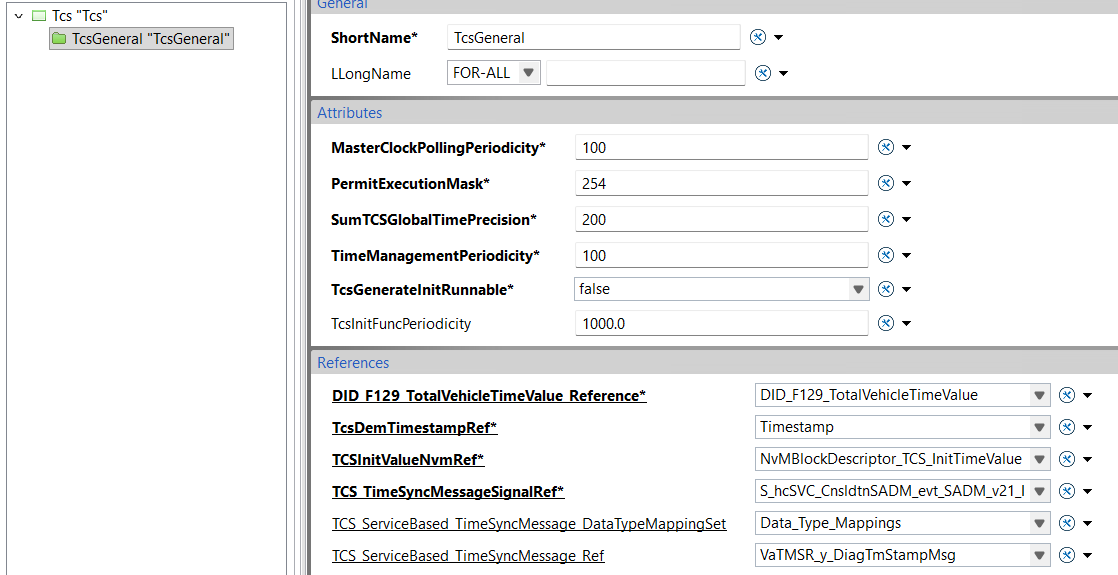
\includegraphics[width=\linewidth]{images/general.png}

\textbf{MasterClockPollingPeriodicity}\newline
It's the time in milliseconds for the periodicity of the Runnable MasterClockPolling which polls Master Clock signal and availability signal and also synchronizes local timer to Master Clock.
Please note that this periodicity value must be less than or equal to the transmission rate of the TimeSyncMessage from TS\_Master.

\textbf{PermitExecutionMask}\newline
Bitmask used to identify the Wakeup bit in the SUSD\_TCS\_PermitExecution interface. The Mask can be OR'd with the value supplied by SUSD\_TCS\_PermitExecution to set any "don't care" bits to '1'.

\textbf{SumTCSGlobalTimePrecision}\newline
Local time source accuracy in milliseconds. Must be a multiple of 100 milliseconds and be greater or equal to TimeManagementPeriodicity.

\textbf{TimeManagementPeriodicity}\newline
It's the time in milliseconds for the periodicity of the Runnable TimeManagement which keeps a local clock source to maintain time between receptions of Master Clock Signal and provides a local clock source.
Please note that this periodicity value must be a submultiple of the resolution of the TimeSyncMessage (100 ms).

\textbf{TcsGenerateInitRunnable}\newline
Defines whether a Runnable shall be generated to call the module's init function.

\textbf{TcsInitFuncPeriodicity}\newline
Defines time in ms for the periodicity of the runnable Runnable\_TCS\_Init.

\textbf{TCS\_TimeSyncMessageSignalRef}\newline
Reference to the ComSignal or ComGroupSignal used for the TimeSyncMessage reception. 
This parameter is mandatory.
\begin{itemize}
	\item \textbf{Service-based} (SOME/IP): reference a \code{ComSignal} with \code{comSignalType = UINT8\_N}.\\[1em]
	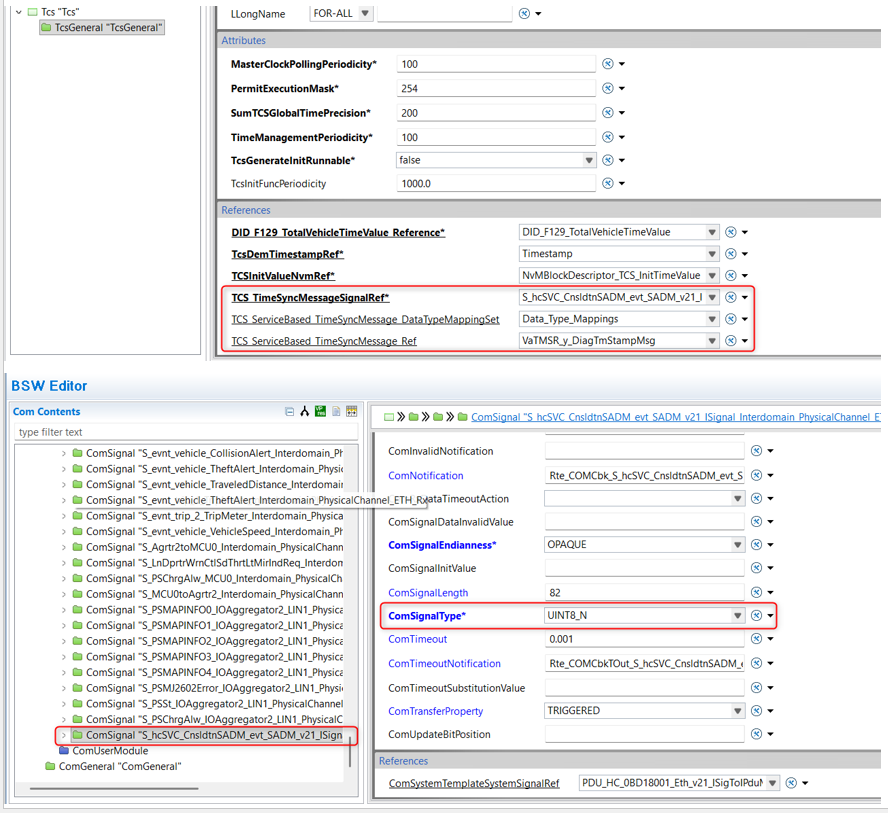
\includegraphics[width=\linewidth]{images/TCS_TimeSyncMessageSignalRef_Servicebased.png}
	\item \textbf{Signal-based}: reference a \code{ComSignal} or \code{ComGroupSignal} with \code{comSignalType = UINT64}.\\[1em]
	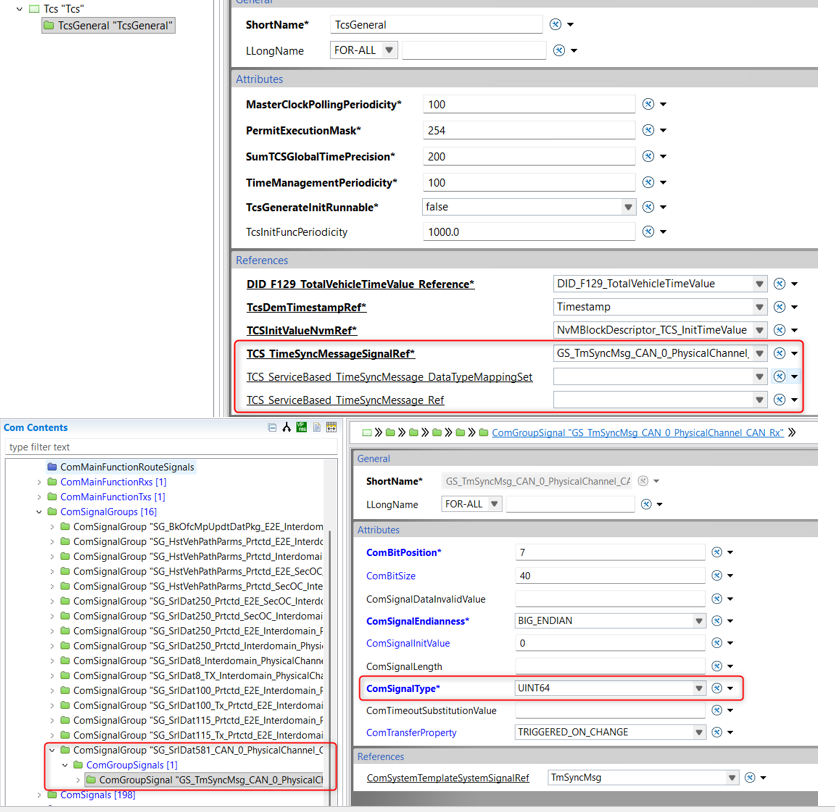
\includegraphics[width=\linewidth]{images/TCS_TimeSyncMessageSignalRef_Signalbased.png}
\end{itemize}
Note: \code{ComGroupSignal} cannot be used for service-based communication.

\textbf{TCS\_ServiceBased\_TimeSyncMessage\_Ref}\newline
Reference to the implementation data type element for service-based TimeSyncMessage communication (e.g. \code{VaTMSR\_y\_DiagTmStampMsg}).
\begin{itemize}
	\item \textbf{Service-based}: configure with a reference to an \code{IMPLEMENTATION-DATA-TYPE-ELEMENT} that has \code{CATEGORY = ARRAY} (byte array).\\[1em]
	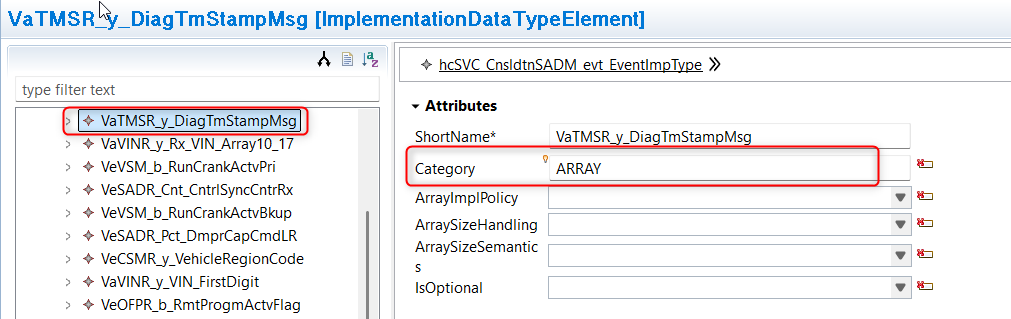
\includegraphics[width=\linewidth]{images/TCS_ServiceBased_TimeSyncMessage_Ref.png}
	\item \textbf{Signal-based}: must \textbf{NOT} be configured.
\end{itemize}
Note: the ARRAY constraint cannot be validated by the generator; referencing a non-array element causes incorrect runtime behavior.

\textbf{TCS\_ServiceBased\_TimeSyncMessage\_DataTypeMappingSet}\newline
Reference to the data type mapping set for service-based communication.
\begin{itemize}
	\item \textbf{Service-based}: required when \code{TCS\_ServiceBased\_TimeSyncMessage\_Ref} is configured.
	\item \textbf{Signal-based}: not needed.
\end{itemize}

\textbf{DID\_F129\_TotalVehicleTimeValue\_Reference}\newline
Reference to DCM DID 0xF129 Total Vehicle Time value

\textbf{TcsDemTimestampRef}\newline
Reference to Dem Timestamp

\chapter{Generic Component Interface}

\begin{center}
	\includegraphics[width=0.7\textwidth,keepaspectratio]{diagrams_generated/Generic_Component_Interface}
\end{center}

\input{generated/tables/port_interfaces.tex}